\documentclass{article}

\usepackage[T1]{fontenc}
\usepackage[utf8]{inputenc}
\usepackage{times}

\usepackage[font=small,labelfont=bf,tableposition=top]{caption}
\usepackage{graphicx}
\usepackage{natbib} 

\usepackage{amsmath}
\usepackage{amsfonts}
\usepackage{amssymb}
\usepackage{color, soul}
\usepackage{hyperref}
\usepackage{algorithmicx}
\usepackage{algpseudocode}
\usepackage{subfigure}
\usepackage{stmaryrd}

\renewcommand{\vec}[1]{\boldsymbol{{#1}}} 
\newcommand{\duesoon}[1]{{\sethlcolor{green}\hl{#1}}}
\usepackage{mathrsfs}


\newtheorem{theorem}{Theorem}
\newtheorem{acknowledgement}[theorem]{Acknowledgement}
\newtheorem{algorithm}[theorem]{Algorithm}
\newtheorem{axiom}[theorem]{Axiom}
\newtheorem{case}[theorem]{Case}
\newtheorem{claim}[theorem]{Claim}
\newtheorem{conclusion}[theorem]{Conclusion}
\newtheorem{condition}[theorem]{Condition}
\newtheorem{conjecture}[theorem]{Conjecture}
\newtheorem{corollary}[theorem]{Corollary}
\newtheorem{criterion}[theorem]{Criterion}
\newtheorem{definition}[theorem]{Definition}
\newtheorem{example}[theorem]{Example}
\newtheorem{exercise}[theorem]{Exercise}
\newtheorem{lemma}[theorem]{Lemma}
\newtheorem{notation}[theorem]{Notation}
\newtheorem{problem}[theorem]{Problem}
\newtheorem{proposition}[theorem]{Proposition}
\newtheorem{remark}[theorem]{Remark}
\newtheorem{solution}[theorem]{Solution}
\newtheorem{summary}[theorem]{Summary}
\newenvironment{proof}[1][Proof]{\textbf{#1.} }{\ \rule{0.5em}{0.5em}}

\newtheorem{guess}{Definition}
\newcommand{\comment}[1] {}
\newcommand{\Norder} {N}
\newcommand{\order}{\mathcal{O}}
\newcommand{\Npoints} {N_p}
\newcommand{\Nfaces} {N_{f}}
\newcommand{\Nelements} {N_e}

\newcommand{\eps}{\varepsilon}
\newcommand{\Dweak}{\wt{D}}
\newcommand{\diff}[2] {\frac{\partial #1}{\partial #2}}
\newcommand{\dxx}[2] {\frac{\partial^2 #1}{\partial {#2}^2}}
\newcommand{\difft}[2] {\frac{d #1}{d #2}}
\newcommand{\dxxt}[2] {\frac{d^2 #1}{d {#2}^2}}
\newcommand{\lagrange}[1] {\frac{d #1}{dt}}
\newcommand{\lebesgue}{\parallel I \parallel}
\newcommand{\polysp}{\mathcal{P}_N}
\newcommand{\laplacian}{\nabla^2}
\newcommand{\divergence}{\nabla \cdot}
\newcommand{\inte}{\int_{\mbox{\footnotesize ${\Omega_e}$}}}
\newcommand{\intb}{\int_{\mbox{\footnotesize ${\Gamma_e}$}}}
\newcommand{\intce}{\int_{\mbox{\footnotesize ${\widehat{\Omega}_e}$}}}
\newcommand{\intcb}{\int_{\mbox{\footnotesize ${\widehat{\Gamma}_e}$}}}
\newcommand{\intg}{\int_{\mbox{\footnotesize ${\Omega}$}}}
\newcommand{\intgb}{\int_{\mbox{\footnotesize ${\Gamma}$}}}
\newcommand{\intv}{\int_{\mbox{\footnotesize ${\sigma}$}}}
\newcommand{\sumv}{\sum_{K=1}^{N_{\mathrm{lev}}}}
\newcommand{\sumk}{\sum_{L=1}^{K}}
\newcommand{\sumN}{\sum_{i=1}^{N+1}}
\newcommand{\half}{\frac{1}{2}}
\newcommand{\inti}{\int_{\mbox{\footnotesize\sf I}}}
\newcommand{\intbd}{\oint_{\mbox{\footnotesize ${\delta}$\sf D}}}
\newcommand{\intbi}{\oint_{\mbox{\footnotesize ${\delta}$\sf I}}}
\newcommand{\ldnorm}[1]{\left\| #1 \right\|_{\mbox{\footnotesize \sf D}} }
\newcommand{\lonorm}[1]{\left\| #1 \right\|_{\Omega}}
\newcommand{\spc}[1]{\mbox{\sf #1}}
\newcommand{\ope}[1]{{\cal #1}}
\newcommand{\mt}[1]{{\rm #1}}
\newcommand{\dis}{\displaystyle}
\newcommand{\ve}{\varepsilon}
\newcommand{\ov}{\overline}
\newcommand{\wt}{\widetilde}
\newcommand{\wh}{\widehat}
\newcommand{\Dhat}{\widehat{D}}
\newcommand{\be}{\begin{equation}}
\newcommand{\ee}{\end{equation}}
\newcommand{\bea}{\begin{eqnarray*}}
\newcommand{\eea}{\end{eqnarray*}}
\newcommand{\Jace}{J^{(e)}}
\newcommand{\Jacl}{J^{(l)}}
\def\bepsilon{\mbox{\boldmath $\epsilon $}}
\def\bpsi{\mbox{\boldmath $\psi $}}
\def\bphi{\mbox{\boldmath $\phi $}}
\def\bmu{\mbox{\boldmath $\mu $}}
\def\Et{ \tilde{E} }
\def\Ht{ \tilde{H} }
\def\sdot{ \dot{\sigma} }

\newcommand{\fstar}{f^{(*)}}

\DeclareMathOperator{\Span}{span}
\DeclareMathOperator{\Dim}{dim}

\newcommand{\polyquad}{\mathcal{Q}_{N}}
\newcommand{\polyP}{\mathcal{P}_{N}}
\newcommand{\polyPnpm}{\mathcal{P}_{(N+M)}}
\newcommand{\polyPd}{\mathcal{P}_{d}}
\newcommand{\polyPnm}{\mathcal{P}_{N,M}}
\newcommand{\polyPn}{\mathcal{P}_{N,0}}
\newcommand{\transpose}{^{\mathcal{T}}}

\newcommand{\vecQ}{\vec{Q}}
\newcommand{\vecQe}{\vec{Q}^{(e)}}
\newcommand{\vecFe}{\vec{\mathcal{F}}^{(e)}}
\newcommand{\statevec}{\vec{Y}}
\newcommand{\statevecN}{\vec{Y}_N^{(e)}}
\newcommand{\statestage}{\vec{\mathcal{Y}}}
\newcommand{\Ftensor}{\vec{F}(\qvector)}
\newcommand{\FtensorN}{\vec{F}\left( \qvectorN \right)}
\newcommand{\FtensorStar}{\vec{F}\left( \qvector_N^{(e,k)} \right)}
\newcommand{\Svector}{S(\qvector)}
\newcommand{\SvectorN}{S \left( \qvectorN \right)}
\newcommand{\qref}{\vec{q}_0}
\newcommand{\qvectorb}{\vec{q}_b}
\newcommand{\qtt}{\vec{q}_{tt}}
\newcommand{\qhat}{\widehat{\vec{q}}}
\newcommand{\qhatb}{\widehat{\vec{q}}_b}
\newcommand{\qelem}{q^{(e)}}
\newcommand{\rhoref}{\rho_0}
\newcommand{\piref}{\pi_0}
\newcommand{\Thetaref}{\Theta_0}
\newcommand{\Gref}{G_0}
\newcommand{\Tref}{T_0}
\newcommand{\thetaref}{\theta_0}
\newcommand{\Pref}{{P}_0}
\newcommand{\Eref}{{E}_0}
\newcommand{\Href}{{h}_0}
\newcommand{\rhohat}{\widehat{\rho}}
\newcommand{\pihat}{\widehat{\pi}}
\newcommand{\Phat}{\widehat{P}}
\newcommand{\uvechat}{\widehat{{\mbox{\boldmath$u$\unboldmath}}}}
\newcommand{\uhathat}{\widehat{\widehat{{\mbox{\boldmath$u$\unboldmath}}}}}
\newcommand{\Uhat}{\widehat{{\mbox{\boldmath$U$\unboldmath}}}}
\newcommand{\Uhathat}{\widehat{\widehat{{\mbox{\boldmath$U$\unboldmath}}}}}
\newcommand{\thetahat}{\widehat{\theta}}
\newcommand{\Thetahat}{\widehat{\Theta}}
\newcommand{\Ehat}{\widehat{E}}
\newcommand{\uhat}{\widehat{u}}
\newcommand{\vhat}{\widehat{v}}
\newcommand{\what}{\widehat{w}}
\newcommand{\pitt}{\pi_{tt}}
\newcommand{\rhott}{\rho_{tt}}
\newcommand{\Ett}{E_{tt}}
\newcommand{\Utt}{\vec{U}_{tt}}
\newcommand{\uvectt}{\vec{u}_{tt}}
\newcommand{\utt}{u_{tt}}
\newcommand{\vtt}{v_{tt}}
\newcommand{\wtt}{w_{tt}}
\newcommand{\Ptt}{P_{tt}}
\newcommand{\vecPtt}{\vec{P}_{tt}}
\newcommand{\Thetatt}{\Theta_{tt}}
\newcommand{\thetatt}{\theta_{tt}}
%Projector Matrices
\newcommand{\projmatrix}{\vec{\mathcal{P}}}
\newcommand{\qmatrix}{\vec{\mathcal{Q}}}
\newcommand{\pcmatrix}{\vec{\mathcal{P}}_C}
\newcommand{\Cmatrix}{\left(\vec{\mathcal{C}}^{(e,f)}\right)\transpose}
\newcommand{\Dmatrix}{\vec{D}^{(e)}}
\newcommand{\Dwmatrix}{\wt{\vec{D}}^{(e)}}
\newcommand{\Mmatrix}{M^{(e)}}
\newcommand{\Fmatrix}{\vec{F}^{(e,l)}}
\newcommand{\Gmatrix}{\mathcal{G}}
\newcommand{\Umatrix}{\mathcal{U}^{(e,f)}}
\newcommand{\amatrix}{\vec{\mathcal{A}}}
\newcommand{\rmatrix}{\vec{\mathcal{R}}}
%Vectors
\newcommand{\nvector}{\wh{\vec{n}}_{\Gamma}}
\newcommand{\nhat}{\wh{\vec{n}}}
\newcommand{\ivector}{\wh{\vec{i}}}
\newcommand{\jvector}{\wh{\vec{j}}}
\newcommand{\kvector}{\wh{\vec{k}}}
\newcommand{\rvector}{\wh{\vec{r}}}
\newcommand{\svector}{\wh{\vec{s}}}
\newcommand{\tvector}{\wh{\vec{t}}}
\newcommand{\vvector}{\wh{\vec{v}}}
\newcommand{\Qvector}{\vec{Q}}
%Vectors
\newcommand{\ur}{{u}^{(r)}}
\newcommand{\us}{{u}^{(s)}}
\newcommand{\ut}{{u}^{(t)}}
\newcommand{\urtt}{{u}_{tt}^{(r)}}
\newcommand{\ustt}{{u}_{tt}^{(s)}}
\newcommand{\uttt}{{u}_{tt}^{(t)}}
\newcommand{\urhat}{\widehat{u}^{(r)}}
\newcommand{\ushat}{\widehat{u}^{(s)}}
\newcommand{\uthat}{\widehat{u}^{(t)}}
%Other Operators
\newcommand{\grad}{\vec{\nabla}}
\newcommand{\Grad}{\vec{\nabla}}
\newcommand{\Dskew}{\mathcal{D}}

\def\bepsilon{\mbox{\boldmath $\epsilon $}}
\def\bpsi{\mbox{\boldmath $\psi $}}
\def\bphi{\mbox{\boldmath $\phi $}}
\def\bmu{\mbox{\boldmath $\mu $}}
\def\Et{ \tilde{E} }
\def\Ht{ \tilde{H} }
\def\sdot{ \dot{\sigma} }
%\renewcommand{\thetable}{\Roman{table}}
%\renewcommand{\thefigure}{\arabic{figure}}

%\DeclareMathOperator{\Span}{span}
%\DeclareMathOperator{\Dim}{dim}

%Editing Commands
\newcommand{\here}{ \textcolor{red}{YOU ARE HERE}}

%Time-Integration
\newcommand{\dt}{{\Delta t}}
\newcommand\ST{\rule[-0.75em]{0pt}{2em}}
\newcommand{\Sfunction}{\mathcal{S}}
\newcommand{\Lfunction}{\mathcal{L}}
\newcommand{\Nfunction}{\mathcal{N}}

%DG Operators
\newcommand{\average}[1]{ \left\{ #1 \right\} }
\newcommand{\jump}[1]{ \llbracket #1 \rrbracket }

%HDG Matrices
\newcommand{\CCmatrix}{\mathcal{C}^{(e,k)}}
\newcommand{\Jmatrix}{\mathcal{J}^{(e,k)}}
\newcommand{\DDmatrix}{\wt{D}^{(e)}}
\newcommand{\SSvector}{\mathcal{S}(q)}
\newcommand{\cghdg}{cg\underline{\hspace{0.15cm}}to\underline{\hspace{0.15cm}}hdg}
%\newcommand{\ul}{\underline{\hspace{0.15cm}}}
\newcommand{\RRmatrix}{\mathcal{R}}

%Clima specific variables
\newcommand{\etotal}{e^{\mathrm{tot}}}
\newcommand{\Etotal}{E^{\mathrm{tot}}}
\newcommand{\Fvector}{\vec{\mathcal{F}}}
\newcommand{\Pvector}{\vec{\mathcal{P}}}
\newcommand{\Fadv}{\vec{\mathcal{F}}^{\mathrm{adv}}}
\newcommand{\Fndf}{\vec{\mathcal{F}}^{\mathrm{ndf}}}
\newcommand{\Fdiff}{\vec{\mathcal{F}}^{\mathrm{diff}}}
\newcommand{\Tvector}{\vec{\mathcal{T}}}
\newcommand{\Source}{\vec{\mathcal{S}}}

\newcommand{\fxg}[1]{\textcolor{cyan}{FXG: #1}}



\title{Design Document for the CLIMA Atmosphere Model} 
\author{ }

\begin{document}

\maketitle
\tableofcontents

\section{Introduction}
\label{sec:introduction}

This document highlights the design specifications for the atmosphere model that is part of the Climate Machine (CLIMA). We refer to this atmosphere model as CLIMA-atmos. The model is designed to run both in a global configuration and in a large-eddy simulation (LES) configuration from the same code base.  

\section{Governing Equations}
\label{sec:governing_equations}

\subsection{Working Fluid and Equation of State}

The working fluid of the atmosphere model is moist, potentially cloudy air, considered to be an ideal mixture of dry air, water vapor, and condensed water (liquid and ice) suspended in clouds. Dry air and water vapor are taken to be ideal gases. The specific volume of the cloud condensate is neglected relative to that of the gas phases (it is a  factor $10^{3}$ less than that of the gas phases). All phases are assumed to have the same temperature and move with the working fluid. However, although the suspended cloud condensates are moving with the fluid, they need not be in thermodynamic equilibrium with the other fluid constituents; out-of-equilibrium phases such as supercooled liquid can exist. Falling condensate (precipitation) is not considered part of the working fluid and is treated separately.

The density of the moist air is denoted by $\rho$. We use the following notation for the mass fractions of the moist air mixture (mass of a constituent divided by the total mass of the working fluid):
\begin{itemize}
\item $q_d$: dry air mass fraction,
\item $q_v$: water vapor specific humidity,

\item $q_l$: liquid water specific humidity,
\item $q_i$: ice specific humidity,
\item $q_c = q_l + q_i$: condensate specific humidity,
\item $q_t = q_v + q_c$: total specific humidity.
\end{itemize}
Because this enumerates all constituents of the working fluid, we have $q_t + q_d = 1$. In Earth's atmosphere, the water vapor specific humidity $q_v$ generally dominates the total specific humidity $q_t$ and is usually $\order(10^{-2})$ or smaller; the condensate specific humidity is typically $\order(10^{-4})$. Hence, water is a trace constituent of the atmosphere, and only a small fraction of atmospheric water is in condensed phases. 

The pressure $p$ of the working fluid is the sum of the partial pressures of dry air and water vapor, both taken to be ideal gases. Neglecting the volume of the condensed phases (but not their masses), this gives $p = \rho (R_d q_d + R_v q_v) T$, where $R_d$ is the specific gas constant of dry air, and $R_v$ is the specific gas constant of water vapor. Since $q_d = 1-q_t$ and $q_v = q_t - q_c$, this can also be written as
\begin{equation}
    p = \rho R_m T,
\label{eq:eos}
\end{equation}
where
\begin{equation}
    R_m = R_d \left[1 + (\eps_{dv}-1)q_t - \eps_{dv} q_c\right]
\label{eq:R_m}
\end{equation}
is the specific gas ``constant'' of moist air (which is not a constant), and $\eps_{dv} = R_v/R_d$ is the ratio of the molar masses of dry air and water vapor ($\eps_{dv} \approx 1.61$). Equations~\eqref{eq:eos} and \eqref{eq:R_m} constitute the equation of state of the working fluid.

\subsection{Mass Balance}

Moist air mass satisfies the conservation equation
\begin{equation}
\diff{\rho}{t} + \divergence \vec{U} = \rho S_{q_t},
\label{eq:governing_equations/mass}
\end{equation}
where $\vec{U}=\rho \vec{u}$ is the mass flux, with the three-dimensional velocity vector $\vec{u}$ understood to be the velocity of the barycenter of the moist air elements. Moist air mass is not exactly conserved where precipitation forms, sublimates, or evaporates, or where water diffuses \citep{Bott08a}. The  right-hand side involves the local source/sink of water mass $S_{q_t}$ owing to precipitation formation, evaporation/sublimation of precipitating hydrometeors (generally provided by a microphysics parameterization such as the Kessler scheme), or diffusion of water. 

The water mass sources/sinks usually are about two orders of magnitude smaller than the other terms in the mass balance. However, there is evidence that their effect is important, e.g., in strongly precipitating tropical cyclones \citep{Qiu93a,Lackmann04a}. They are zeroth-order important in some other planetary atmospheres, in which the condensable species is a major constituent of the atmosphere. For example, CO\textsubscript{2} is the primary constituent of Mars' atmosphere and seasonally condenses onto the winter pole, leading to large effects of mass non-conservation on the flow \cite[e.g.,][]{Soto15a}. Since we want to be able to use CLIMA-atmos for other planetary atmospheres, we are taking such mass sources/sinks into account.

\subsection{Moisture Balances}

Total water satisfies the conservation equation
\begin{equation}
\diff{(\rho q_t)}{t} + \divergence (q_t \vec{U}) = \rho S_{q_t}.   
\label{eq:governing_equations/moisture}
\end{equation}
The right-hand side is the same as that in the conservation law \eqref{eq:governing_equations/mass} for total mass, which means that the dry air mass $(1-q_t)\rho$ is exactly conserved, and deviations from conservation of the moist air mass $\rho = (1-q_t)\rho + q_t \rho$ arise from deviations from conservation of total water $q_t\rho$. The conservation laws for mass \eqref{eq:governing_equations/mass} and total water \eqref{eq:governing_equations/moisture} together imply the material derivative $dq_t/dt = (1-q_t) S_{q_t}$, with the factor $(1-q_t)$ arising because both the density of moist air $\rho$ and the density of water $\rho_t$ enter $q_t = \rho_t/\rho$, and both change simultaneously when $S_{q_t}$ is nonzero.

The sources/sink of total water can be written as  
\begin{equation}
     \rho S_{q_t} = - \rho C(q_t \rightarrow q_p) - \divergence (\rho \vec{d}_t),
\end{equation}
with evaporation or sublimation of precipitation and formation of precipitation contributing to the conversion from $q_t$ to $q_p$ (i.e., $C(q_t \rightarrow q_p)$), and diffusive and SGS turbulent fluxes of moisture captured by $\vec{d}_t$. The diffusive flux of water consists of fluxes of water vapor, cloud liquid, and cloud ice: $\vec{d}_t =\vec{d}_v + \vec{d}_l + \vec{d}_i$ \citep{Romps08a}.

If the suspended condensates (cloud liquid and ice) are in local thermodynamic equilibrium with the gas phase, Gibbs' phase rule implies that their specific humidities, $q_l$ and $q_i$, can be determined by ``saturation adjustment'' from three other thermodynamic state variables, such as density $\rho$, total water specific humidity $q_t$, and an internal energy variable. However, to enable the explicit modeling of out-of-equilibrium phases (e.g., supersaturated water vapor in the upper troposphere or supercooled liquid water in mixed-phase clouds), we explicitly model the specific humidities of suspended liquid ($q_l$) and ice ($q_i)$. They satisfy conservation equations of the form
\begin{equation}
\diff{(\rho q_k)}{t} + \divergence (q_k \vec{U}) = \rho S_k  -\divergence (\rho \vec{d}_{k}),   
\label{eq:governing_equations/condensate}
\end{equation}
where $k \in \{l, i\}$, 
\begin{align}
    S_l & = C(q_i \rightarrow q_l) + C(q_v \rightarrow q_l) + C(q_p \rightarrow q_l), \\
    S_i & = C(q_l \rightarrow q_i) + C(q_v \rightarrow q_i) + C(q_p \rightarrow q_i)
\end{align}
represent sources of cloud liquid and ice, and $\vec{d}_{k}$ represents diffusive or SGS turbulent fluxes of phase $k$. The terms $C(q_j \rightarrow q_{l/i}) = - C(q_{l/i} \rightarrow q_j)$ represent the conversion of species $j \in \{l, i, v, p\}$ to cloud liquid $q_l$ or cloud ice $q_i$, with $q_p$ representing the mass fraction of precipitation. The conversion terms include processes such as evaporation or sublimation of cloud condensate, melting of cloud ice, or precipitation formation, all provided by microphysics parameterizations. The conversion term $C(q_t \rightarrow q_p) = -C(q_p \rightarrow q_t)$ in equation \eqref{eq:governing_equations/moisture} for total water is the sum of the conversion terms $C(q_l \rightarrow q_p)=-C(q_p \rightarrow q_l)$ and $C(q_i \rightarrow q_p)=-C(q_p \rightarrow q_i)$ from liquid and ice to precipitation, plus an analogous term, $C(q_v \rightarrow q_p)=-C(q_p \rightarrow q_v)$, for the conversion of vapor to precipitation. 
 

\subsection{Momentum Balance}

The vector invariant form of the momentum equation in a coordinate system rotating with constant angular velocity $\vec{\Omega}$ is 
\begin{equation}
\diff{\vec{U}}{t} + \divergence \left( \frac{\vec{U} \otimes \vec{U} }{\rho} + p \vec{I}_3\right) =  - \rho \grad\Phi - 2\vec{\Omega} \times \vec{U} - \divergence \vec{\tau} - \divergence\left( \vec{d}_t \otimes \vec{U} \right)
\label{eq:governing_equations/momentum}
\end{equation}
where $\vec{I}_3$ is the rank-3 identity matrix; $\Phi$ is the effective gravitational potential (including centrifugal accelerations); and $\vec{\tau}$ is a viscous and/or SGS turbulent stress tensor (momentum flux) which is typically defined as follows
\begin{equation}
\vec{\tau}  =  \nabla \vec{u} +  \left( \nabla \vec{u} \right)^T + \lambda \nabla \cdot \vec{u}
\label{eq:governing_equations/momentum/viscous_fluxes}
\end{equation}
where the superscript $T$ represents the transpose operator and the constant $\lambda$ is derived from Stokes' hypothesis.
Mechanical interactions between falling precipitation and the fluid, giving rise to frictional drag on the fluid in shear zones around falling hydrometeors \citep{Pauluis00}, are taken to be included in the stress tensor $\vec{\tau}$. Momentum and kinetic energy transport by precipitating hydrometeors is neglected; it is 3--4 orders of magnitude smaller than other terms in the budgets \citep{Romps08a}.

These are the general, deep-atmosphere equations for a moist, nonhydrostatic atmosphere, without the thin-shell approximation traditionally made in climate models. (The thin-shell approximation assumes that in the formulation of the angular momentum, the distance from any point in the atmosphere to the barycenter of the planet is a constant and equal to the mean planetary radius.)

\subsection{Energy Balance}

To close the equations of motion for the working fluid, we require a thermodynamic or energy balance equation. Various choices are possible, a temperature (internal energy or enthalpy) equation being most common in climate models. We instead use the total specific energy $e^\mathrm{tot}$ to close the system, as in \citet{Romps08a}, a quantity that is conserved in reversible moist processes such as phase transitions of water. 

Total energy satisfies the conservation law \citep{Romps08a}
\begin{multline}
 \diff{(\rho e^{\mathrm{tot}})}{t} + \divergence \left[\vec{U} \left(e^{\mathrm{tot}} + \frac{p}{\rho}\right) \right] 
 = -\divergence (\rho \vec{F}_R)   \\
  - \divergence (\vec{u} \cdot \vec{\tau)} - \divergence (\rho \vec{J}) - \divergence (\rho \vec{D})\\
   - \sum_{j\in\{v,l,i\}}(I_j + \Phi)  \rho C(q_j \rightarrow q_p) - M,
 \label{eq:energy_balance}
\end{multline}
where the total specific energy is the weighted sum of the total specific energies of the moist air constituents (dry air, water vapor, cloud liquid, cloud ice):
\begin{equation}
    e^{\mathrm{tot}} = (1-q_t) e_d^{\mathrm{tot}} + q_v e_v^{\mathrm{tot}} + q_l e_l^{\mathrm{tot}} + q_i e_i^{\mathrm{tot}}.
\end{equation}
Each constituent is assumed to be moving with the same velocity and to have the same temperature, so that the constituent specific energies can be written as
\begin{align}
e_d^{\mathrm{tot}} & = \frac{1}{2} \| \vec{u} \|^2 + \Phi + I_d(T), \qquad & I_d(T) & = c_{vd} (T - T_0)  \\
e_v^{\mathrm{tot}} & = \frac{1}{2} \| \vec{u} \|^2 + \Phi + I_v(T), \qquad & I_v(T) & = c_{vv} (T - T_0) + I_{v,0}\\
e_l^{\mathrm{tot}} & = \frac{1}{2} \| \vec{u} \|^2 + \Phi + I_l(T), \qquad & I_l(T) & = c_{vl} (T - T_0) \\
e_i^{\mathrm{tot}} & = \frac{1}{2} \| \vec{u} \|^2 + \Phi + I_i(T), \qquad & I_i(T) & = c_{vv} (T - T_0)  - I_{i,0}.
\end{align}
The total specific energy of each constituent consists of the kinetic energy per unit mass, gravitational potential energy per unit mass $\Phi$, and the specific internal energy $I_k$ ($k \in \{d, v, l, i\}$). Here, $c_{vx}$ are the isochoric specific heat capacities of the constituents $x$, taken to be constant;  $T_0$ is a reference temperature, $I_{v,0}$ is the difference in specific internal energy between vapor and liquid at $T_0$, and $I_{i,0}$ is the difference in specific internal energy between ice and liquid at $T_0$. After summation over the constituents, the total specific energy of moist air becomes
\begin{equation}
     e^{\mathrm{tot}} = \frac{1}{2} \| \vec{u} \|^2 + \Phi + I,
     \label{eq:total_energy_def}
\end{equation}
where 
\begin{equation}
     I(T) = c_{vm} (T - T_0)  + q_v I_{v,0} - q_i I_{i,0}
     \label{eq:total_internal_energy}
\end{equation}
is the specific internal energy of the moist air, with the isochoric specific heat capacity of moist air $c_{vm} = (1-q_t) c_{vd} + q_v c_{vv} + q_l c_{vl} + q_i c_{vi}$.

On the right-hand side of \eqref{eq:energy_balance}, the flux $\vec{F}_R$ is the radiative energy flux per unit mass, and $\vec{J}$ is the conductive or SGS turbulent flux of sensible heat per unit mass. The flux 
\begin{equation}
\vec{D} = (e_v^{\mathrm{tot}} + R_v T) \vec{d}_v + e_l^{\mathrm{tot}} \vec{d}_l +  e_i^{\mathrm{tot}} \vec{d}_i
\end{equation}
is the total specific energy flux (plus the term $p_v/\rho = R_v T$ involving the partial pressure of water vapor $p_v$ for the gas phase) owing to the diffusive or SGS turbulent flux of water. The terms involving $\rho C(q_j \rightarrow q_p)$ ($j \in \{ v, l, i \}$) represent the loss of internal and potential energy of moist air masses owing to precipitation formation; the kinetic energy loss is neglected consistent with the neglect of the source/sink associated with precipitation formation in the momentum balance \eqref{eq:governing_equations/momentum}. Additional energy sinks involve the energy loss owing to heat transfer from the working fluid to precipitation as it falls through it and possibly melts at the freezing level \citep{Raymond13b}; the associated energy sources/sinks are provided by a microphysics parameterization and are subsumed in the term $M$.

The temperature can be recovered from the definition \eqref{eq:total_internal_energy} of internal energy $I = e^{\mathrm{tot}} - 0.5 \| \vec{u} \|^2 - \Phi$  as 
\begin{equation}
    T = T_0 + \frac{I - (q_t - q_l) I_{v,0} + q_i (I_{i,0} + I_{v,0})}{c_{vm}},
    \label{eq:temperature}
\end{equation}
where we have used $q_v = q_t - q_l - q_i$. The pressure $p$ can then be computed from the ideal gas law \eqref{eq:eos}. The equations \eqref{eq:eos}--\eqref{eq:temperature} form the governing equations of the moist atmosphere.

Note that latent heating as a result of phase changes of water redistributes energy among terms in the definition of total energy, but it does not appear as a source term on the right-hand side of the energy balance \eqref{eq:energy_balance}. Therefore, a dry dynamical core can easily be converted into a moist dynamical core simply by adapting the definition of internal energy to include moisture variables. The right-hand sides only need to change to account for irreversible processes such as diffusion of water vapor or precipitation formation. 

The internal energy terms in the total energy of Earth's atmosphere are typically about two orders of magnitude larger than the kinetic energy terms: Because the speed of sound in an ideal gas is $c_s = \sqrt{(c_p/c_v) R T}$, the internal energy is of order $c_s^2 \approx (330~\mathrm{m~s^{-1}})^2 \approx 110000~\mathrm{m^2~s^{-2}}$, which is two orders of magnitude greater than the kinetic energy $0.5 \|\vec{u}\|^2 \lesssim 0.5(40~\mathrm{m~s^{-1}})^2 = 800~\mathrm{m^2~s^{-2}}$. This means that the magnitudes of total energy and internal energy are of the same order - this implies that the truncation error in mapping from total energy to temperature should not be severe.

Thermodynamic quantities appearing here, such as the specific heats and the specific internal energies at a reference temperature, will be discussed further in section~\ref{s:thermodynamics}.

\subsection{Precipitation}

We  consider $N_p$ species of precipitation (e.g., rain, snow, graupel), with specific humidities $q_{p,i}$ ($i=1,\dots,N_p$). Precipitation species $i$ falls with a fall velocity $w_i$ (approximately the terminal velocity of falling hydrometeors), which is defined to be positive downward. With the upward vertical unit vector $\vec{k}$, the conservation equation for the precipitation species $i$ then becomes
\begin{equation}
\diff{(\rho q_{p,i})}{t} + \divergence \left[q_{p,i} (\vec{U} - \rho w_i \vec{k}) \right] = \rho \left[C(q_t \rightarrow q_{p,i}) + C(q_{p,k} \rightarrow q_{p,i}) \right],   
\label{eq:precip}
\end{equation}
where $C(q_t \rightarrow q_{p,i})$ represents the conversion of suspended total water to precipitation species $i$, and $C(q_{p,k} \rightarrow q_{p,i}) = -C(q_{p,i} \rightarrow q_{p,k})$ represents the conversion of precipitation species $k$ to $i$. 

In principle, the temperature of the precipitation species can differ from the ambient temperature (e.g., the wet bulb temperature can be a good approximation). If that is to be taken into account, an additional temperature tracer for each precipitation species is also needed.

\subsection{Tracers}

We also allow $N_\chi$ passive tracers $\chi_i$ ($i=1, \dots, N_\chi$), each satisfying balance laws
\begin{equation}
\diff{(\rho \chi_i)}{t} + \divergence \left(\chi_i \vec{U} \right) = \rho S_{\chi_i},   
\label{eq:tracers}
\end{equation}
with sources/sinks $S_{\chi_i}$. Note that the mass sink associated with precipitation on the right-hand side of the continuity equation \eqref{eq:governing_equations/mass} implies that the material derivative of the tracer is $D\chi_i/Dt = S_{\chi_i} - \chi S_{q_t}$.
 
\subsection{Boundary Conditions}

\paragraph{Top.} At the top of the atmosphere, we require a boundary that absorbs upward propagating waves. This is commonly accomplished by the introduction of sponge layers at a rigid model lid. However, sponge layers often lead to non-conservation of angular momentum and imply unphysical zonal-mean torques exerted by the atmosphere on outer space. These can lead to artifacts and biases in the circulation of the model's upper atmosphere \citep[e.g.,][]{Shepherd96a}.

\hl{Frank: Your thoughts here would be appreciated. How do we formulate the upper boundary, ideally so that the atmosphere model can be easily made into an ocean model (i.e., with a free surface)? In usual discretizations, the choice of upper boundary affects energy conservation} \citep[e.g.,][]{Staniforth03a}, \hl{but probably that disappears as a problem when energy is a prognostic variable}.

\hl{Tapio: This is tricky and I will need to talk to the Ocean modeling group about this.  I believe John told me that the way they will handle a free surface is through the inclusion of another variable (eta) which is the free surface boundary. For atmosphere, I assume we just need some radiative BC at the top; however, as you state above, this will affect conservation so let me propose what I write here below. However, both of these approaches below only handle the atmosphere - not sure what to do with the ocean.}
One possible approach, which is typically used in Godunov methods, is to use an extrapolation condition whereby the Riemann solver is modified in order to let flow move out of the domain.  Another possibility is to use an approach recently proposed by Benacchio and Bonaventura whereby they use Laguerre functions in a DG approach to enforce absorbing boundary conditions (see \texttt{https://arxiv.org/pdf/1803.10997.pdf}).


\paragraph{Bottom.} At the bottom boundary, Monin-Obukhov similarity theory is typically used for modeling the exchange of momentum, heat, water vapor, and tracers between the surface and the lowest model level. Care must be taken to formulate this accurately for finite-volume discretizations  \citep{Nishizawa18a}.

\paragraph{Lateral.} Lateral boundary conditions do not arise on the sphere. However, several forms of lateral boundary conditions arise in LES configurations: We want to be able to configure the model
\begin{itemize}
    \item with horizontally doubly periodic boundary conditions,
    \item in a re-entrant channel configuration with impenetrable walls on two sides, and 
    \item with absorbing horizontal boundary conditions (e.g., relaxation to a global-model state on a coarse grid). 
\end{itemize}

\subsection{Coordinate Systems}

Expressing the equations of motion in spherical coordinates may be convenient for some purposes. The transformation of differential operators to spherical coordinates is straightforward for all scalar conservation laws. For the vector-valued momentum balance, additional (``metric'') terms arise from derivatives of the rotating coordinate basis vectors. The transformation of the three components of the momentum balance \eqref{eq:governing_equations/momentum} to spherical coordinates is standard \citep[e.g.,][]{Staniforth03a}. We will consider whether we want to adopt spherical coordinates later. 

\subsection{Model Configurations.} The model will need to be capable of running in a global climate model configuration and in a regional LES configuration. Ideally, it would solve the same equations of motion in either configuration and at any resolution. This would require SGS process models in the global model that are scale-aware and reduce to LES SGS models (or no SGS models for implicit LES) at high resolution. This may not be feasible to achieve immediately. Thus, we will need easy ways to configure SGS models for global and LES configurations of the model. 

The global model needs to be able to spin-off high-resolution LES (with around $10^6$ degrees of freedom each) on demand, at locations that need to be addressable from the DA/ML layer of CLIMA. Parameterizations in the global model will learn from these high-resolution simulations. 

\section{Moist Thermodynamics}\label{s:thermodynamics}

The thermodynamics of moist air is often subject to empirical approximations, which usually are opaque, internally inconsistent, and/or inconsistent across model components. For example, microphysical process models often use different approximations for thermodynamic quantities such as saturation vapor pressures than the dynamical core. The often bewildering array of approximations makes it difficult to achieve global conservation, e.g., of energy, and it complicates the use of models for other planetary atmospheres, with different thermodynamic parameters. 

Here we employ one consistent set of thermodynamic approximations for all model components. These result in straightforward, easily adaptable, and relatively accurate expressions for thermodynamic quantities, including closed-form expressions of saturation vapor pressures in terms of thermodynamic parameters. The key to thermodynamic consistency at reasonable accuracy is to take the specific heat capacities of the constituents of moist air (dry air, water vapor, liquid water, and ice) to be constant. All other thermodynamic quantities can then be derived \citep[cf.][]{Romps08a}. 

\subsection{Heat Capacities}\label{s:heat_capacities}

The isochoric specific heat capacities of the constituents of moist air are:
\begin{enumerate}
    \item $c_{vd}$: Isochoric specific heat capacity of dry air;
    \item $c_{vv}$: Isochoric specific heat capacity of water vapor;
    \item $c_{vl}$: Isochoric specific heat capacity of liquid water;
    \item $c_{vi}$: Isochoric specific heat capacity of ice.
\end{enumerate}
We take these isochoric specific heat capacities to be constants. This is an approximation because they depend weakly on temperature. But for atmospheric conditions, the error of approximating them as constant is less than 1\% for dry air, the main constituent of moist air, and at most a few percent for the water phases.

The difference between the isochoric and isobaric specific heat capacities is proportional to the specific volume. Consistent with taking the specific volume of liquid water and ice to be zero, we take the isochoric and isobaric specific heat capacities of the condensed phases to be equal. The isobaric specific heat capacities of the constituents then are:
\begin{enumerate}
    \item $c_{pd} = c_{vd} + R_d$: Isobaric specific heat capacity of dry air;
    \item $c_{pv} = c_{vv} + R_v$: Isobaric specific heat capacity of water vapor;
    \item $c_{pl} = c_{vl}$: Isobaric specific heat capacity of liquid water;
    \item $c_{pi} = c_{vi}$: Isobaric specific heat capacity of ice.
\end{enumerate}

The corresponding specific heat capacities of moist air are the weighted sum of those of the constituents:
\begin{align}
    c_{x m} & = (1-q_t) c_{\cdot d} + q_v c_{\cdot v} + q_l c_{\cdot l} + q_i c_{\cdot i}\\
    & = c_{\cdot d} + (c_{\cdot v} - c_{\cdot d})q_t + (c_{\cdot l} - c_{\cdot v})q_l + (c_{\cdot i} - c_{\cdot v})q_i
\end{align}
where $\cdot$ stands for $v$ or $p$ and we have used $q_v = q_t -q_l - q_i$.

\subsection{Latent Heats}

Kirchoff's relation states that the specific latent enthalpy (heat) $L$ of a phase change depends on temperature $T$ through
\begin{equation}
    \frac{dL}{dT} = \Delta c_p,
\end{equation}
where $\Delta c_p$ is the difference in isobaric specific heat capacities between the phase with the higher specific volume and that with the lower specific volume. For the constant isobaric specific heat capacities that we assume, this can be integrated to give
\begin{equation}
    L = L_0 + \Delta c_p (T-T_0),
    \label{eq:LH_temperature}
\end{equation}
where $T_0$ is a reference temperature and $L_0$ is the latent heat at $T_0$. 

For the phase transitions of water, this implies specifically:
\begin{enumerate}
    \item $L_v = L_{v,0} + (c_{pv} - c_{pl}) (T - T_0)$: Latent heat of vaporization;
    \item $L_f = L_{f,0} + (c_{pl} - c_{pi}) (T - T_0)$: Latent heat of fusion;
    \item $L_s = L_{s,0} + (c_{pv} - c_{pi}) (T - T_0)$: Latent heat of sublimation.
\end{enumerate}

\subsection{Reference Internal Energies}

The specific internal energy \eqref{eq:total_internal_energy} requires the difference in specific internal energy between vapor and liquid and between liquid and ice, both at the reference temperature $T_0$. 

The specific latent heats $L_{v,0}$, $L_{f,0}$, and $L_{s,0}$ give the enthalpy difference between the phases at $T_0$. The specific internal energy differences are obtained by subtracting the ``$pV$'' term, which is $p_\cdot/\rho_\cdot$ for the relevant partial pressure $p_\cdot$ and specific volume $1/\rho_\cdot$. This gives
\begin{align}
     I_{v,0} &= L_{v, 0} - R_v T_0,\\
     I_{i,0} &= L_{f, 0},
\end{align}
where we again neglected the specific volume of the condensed phases. 
   
\subsection{Saturation Vapor Pressure}

The Clausius-Clapeyron relation describes how the saturation vapor pressure $p_v^*$ of an ideal gas over a plane surface of condensate depends on temperature:
\begin{equation}
    \frac{d \log(p_v^*)}{dT} = \frac{L}{R_v T^2}.
\end{equation}
Here, $L$ is the latent heat of the phase transition, which may be $L_v$ for the saturation vapor pressure over liquid, or $L_s$ for the saturation vapor pressure over ice. Substituting the linear relation \eqref{eq:LH_temperature} between latent heat and temperature, and taking $p_\mathrm{tr}$ to be the vapor pressure at the triple point (by definition equal to the saturation vapor pressures both over liquid and ice), the Clausius-Clapeyron relation can be integrated to give a closed-form expression for the vapor pressure that is consistent with our thermodynamic assumptions:
\begin{equation}
    p_v^* = p_{\mathrm{tr}} \left( \frac{T}{T_{\mathrm{tr}}} \right)^{\frac{\Delta c_p}{R_v}}
        \exp \left[ \frac{L_0 - \Delta c_p T_0}{R_v} 
        \left( \frac{1}{T_{\mathrm{tr}}} - \frac{1}{T} \right) \right].
        \label{eq:sat_vapor_pressure}
\end{equation}
With $L_0 = L_{v,0}$ or $L_0 = L_{s,0}$ and the corresponding heat capacity difference $\Delta c_p$, this gives saturation vapor pressures over liquid or ice that are accurate within 3\% for temperatures between 200 and 330~K (with accuracy better than 1\% for typical near-surface conditions).

To obtain the saturation vapor pressure over a mixture of liquid and ice (e.g., in mixed-phase clouds), using a weighted average of the relevant specific latent heats in the vapor pressure \eqref{eq:sat_vapor_pressure} leads to a thermodynamically consistent formulation \citep{Pressel15a}. That is, if a fraction $\lambda$ of the condensate is liquid and the complement $1-\lambda$ is ice, calculating the saturation vapor pressure with a latent heat $\lambda L_v + (1-\lambda)L_s$ gives a thermodynamically consistent saturation vapor pressure over the mixture. In thermodynamic equilibrium, the liquid fraction $\lambda(T) = \mathcal{H}(T-T_{\mathrm{freeze}})$ is a Heaviside function $\mathcal{H}$ of temperature, being zero 0 below the freezing temperature $T_{\mathrm{freeze}}$ and 1 above it. However, out of thermodynamic equilibrium, supercooled liquid can exist between the temperature of homogeneous ice nucleation and the freezing temperature.

\subsection{Saturation Specific Humidity}

From the saturation vapor pressure $p_v^*$, the saturation specific humidity can be computed using the ideal gas law, giving the density of water vapor at saturation $\rho_v^* = p_v^*(T)/(R_v T)$, and hence the saturation specific humidity 
\begin{equation}\label{eq:sat_shum}
     q_v^* = \frac{\rho_v^*}{\rho} = \frac{p_v^*(T)}{\rho R_v T}.
\end{equation}

\subsection{Saturation Adjustment}

Gibbs' phase rule states that in thermodynamic equilibrium, the temperature $T$ and liquid and ice specific humidities $q_l$ and $q_i$ can be obtained from the three thermodynamic state variables density $\rho$, total water specific humidity $q_t$, and internal energy $I$. Thus, a moist dynamical core that assumes equilibrium thermodynamics can be obtained from a dry dynamical core with total energy as a prognostic variable by including only a tracer for the total specific humidity $q_t$, and calculating the temperature and condensate specific humidities from $\rho$, $q_t$, and $I$. 

Because the temperature \eqref{eq:temperature} depends on the condensate specific humidities at saturation (equilibrium), which in turn depend on temperature, obtaining the temperature and condensate specific humidities from the other state variables is a nonlinear problem. This nonlinear problem must be solved iteratively, in what is known as a saturation adjustment procedure. Saturation adjustment proceeds by calculating the internal energy at saturation $I^*(T; \rho, q_t)$ and then finding the zero of $I-I^*(T; \rho, q_t)$ as a function of temperature $T$. The internal energy at saturation is obtained from the saturation specific humidity \eqref{eq:sat_shum}, which determines the condensate specific humidity $q_c = \max(q_t - q_v^*, 0)$, and then partitioning the condensate specific humidity according to the liquid fraction $\lambda(T)$ into liquid $q_l = \lambda q_c$ and ice $(1-\lambda)q_c$. 

Using saturation adjustment allows a moist dynamical core that has the total specific humidity $q_t$ as the only prognostic moisture variable. The price for this simplicity is the necessity to solve a nonlinear problem iteratively at each time step, and being confined to an equilibrium thermodynamics framework. Using explicit tracers for the condensates $q_l$ and $q_i$ in addition to $q_t$ avoids iterations at each time step and allows the inclusion of explicit non-equilibrium processes, such as those leading to the formation of supercooled liquid in mixed-phase clouds. 


\section{Numerical Methods}
\label{sec:numerical_methods}

\hl{[Please include the moisture equations here along with the dry equations, and make notation and rhs's consistent with section~1.]}

In order to describe the numerical methods used to solve the governing equations numerically, let us write the equations in the following compact form \hl{[need tracers for $q_t$, $q_l$, $q_i$, and others $\chi_i$ for chemistry]}
\[
\diff{\vec{Q}}{t} = - \nabla \cdot \left( \vec{F}^{inv} - \vec{F}^{visc} \right) + \mathcal{S}(\vec{Q})
\]
where \hl{[define $E = \rho e^{\mathrm{tot}}$ here or above, make equations here consistent with above]}
\[
\vec{Q}=\left( \begin{array}{c}
\rho \\
\vec{U} \\
 E\\
\rho \vec{q}\\
\end{array}
\right)
\]
 is the solution vector, 
 \[
 \vec{F}^{inv}=\left( \begin{array}{c}
 \vec{U} \\
 \frac{\vec{U} \otimes \vec{U}}{\rho} + p \vec{I}_3 \\
\frac{(E+p) \vec{U}}{\rho}\\
\frac{\vec{q} \otimes \vec{U}}{\rho}
\end{array}
\right)
 \]
 \hl{[Why the Kronecker product in the moisture equation? Also it is odd to use the specific humidity $q$ as a primitive variable, but then use energy per unit volume $E$ (rather than per unit mass $e^\mathrm{tot}$) as primitive variable. Let's make this consistent.]} is the inviscid flux tensor, 
 \[
 \vec{F}^{visc}=\left( \begin{array}{c}
 \rho\vec{d} \\
 \vec{F}_u \\
\vec{u} \cdot \vec{F}_u + \frac{\mu c_p}{\mathrm{Pr}} \nabla T\\
\rho\vec{d}
\end{array}
\right)
 \] \hl{[leave the sensible heat flux more open--we will not want to diffusive temperature here. Just use $\vec{J}$ as in section~2, and also include the other flux terms symbolically]} is the viscous flux tensor, and
 \[
 \mathcal{S}(\vec{Q})= - \left( \begin{array}{c}
 -\rho C(q_t \rightarrow q_p) \\
 2 \vec{\Omega} \times \vec{U} + \rho g \vec{r} \\
 \sum_{j\in\{v,l,i\}}(I_j + \Phi)  \rho C(q_j \rightarrow q_p) - M \\
-\rho C(q_t \rightarrow q_p)
\end{array}
\right)
 \]
contains the source terms \hl{[Note that the diffusive fluxes and source/sink terms for mass and total moisture are the same--we should make this clearer here, and also in the code: no need to re-type.]}. The viscous stresses for the momentum are defined as \hl{[leave this more open--we will want other SGS closures, e.g., with state-dependent viscosities/diffusivities, Prandtl numbers etc.]}
\[
\vec{F}_u = \mu \left[ \vec{u} + \left( \nabla \vec{u} \right)^T + \lambda \nabla \cdot \vec{u} \vec{I}_3 \right].
\]
In the above flux definitions, $\mathrm{Pr}$ denotes the turbulent Prandtl number, $\lambda$ comes from Stokes hypothesis, and $\mu$ is the dynamic viscosity, which is used for the SGS closures for the LES model.

\subsection{Spatial Discretization Methods}

\subsubsection{Overview}
For the spatial discretization methods, we propose to use variants of the discontinuous Galerkin (dG) method with a tensor-product bases (see, e.g., \citet{giraldo:2008a, abdi:2016}). That is, we propose to use hexahedral (cube) elements in three dimensions.  The nodal tensor-product dG methods are extremely accurate and efficient.  For example, using a basis comprised of $N$th degree Lagrange polynomials results in approximately an accuracy of $\order(\Delta x^{N+1})$. Furthermore, using inexact integration results in a per-element complexity of $\order(N^{d+1})$ for constructing derivatives, where $d$ denotes the dimension of the space. 

For the LES model, we will also consider fully three-dimensional dG methods. For the global model, it may be beneficial to consider a hybrid approach whereby the horizontal direction (along the spherical manifold) uses dG while a more standard method (open for discussion) may be used in the vertical.  Along certain directions, it may be advantageous to use uniform grid resolution in order to take advantage of larger time-steps (e.g., in using uniform grids for the global or LES model along the vertical direction would allow for some of the grid aspect ratio stiffness to be reduced).  \textbf{FXG: Need references}.

\subsubsection{DG Basics}

\begin{figure}[htbp]
\begin{center}
\subfigure[Global Domain]{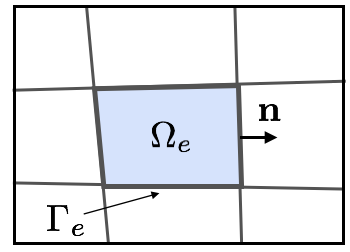
\includegraphics[width=1.5in]{DG_domain.png}
\label{fig:spatial_discretization/dg_domain}}
\subfigure[Element $\Omega_e$]{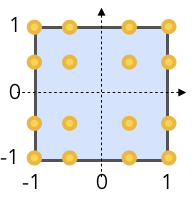
\includegraphics[width=1.5in]{DG_element.png}
\label{fig:spatial_discretization/dg_element}}
\end{center}
\caption{The (a) global domain and (b) element ($N=3$) for the DG method.}
\label{fig:spatial_discretization/dg_method}
\end{figure}

To construct discrete approximations of continuous differential operators (e.g., gradient, divergence, or curl) with the DG method, we first must represent the solution vector (call it $q$) using a polynomial representation.  That is, we represent the solution vector inside of each element $\Omega_e$ as follows
\be
q^{(e)}_N(\vec{x},t) = \sum_{i=1}^{M_N} \psi_i(\vec{x}) q^{(e)}_i(t)
\label{eq:spatial_discretization/dg_method}
\ee
where $\psi(\vec{x})$ are the known basis functions and $q^{(e)}_i(t)$ is the solution at each degree of freedom which will be time-dependent.
The superscript $(e)$ represents the specific element we are working with, $i=1,\ldots,M_N$ represents degrees of freedom inside each element $\Omega_e$.  Figure \ref{fig:spatial_discretization/dg_domain} shows a sample global domain whereby we then identify one specific element $\Omega_e$ to work with.  We then map the element from its physical space to the reference element presented in Fig.\ \ref{fig:spatial_discretization/dg_element}; in this particular example $M_N=(N+1)^2$ where $N=3$ which means we are using 3rd degree polynomials in each direction (yielding 4th degree accuracy).  In general, $N$ need not be constant in each direction and so we can also write $M_N=(N_{\xi}+1)(N_{\eta}+1)$ in two dimensions or $M_N=(N_{\xi}+1)(N_{\eta}+1)(N_{\zeta}+1)$ in three dimensions, where $\xi$ is along the horizontal direction, $\eta$ along the vertical, and $\zeta$ coming out of the page. 

The attraction of using basis functions $\psi$ to represent the solution $q$ is that computing the gradient of $q$ now only requires applying the gradient operator directly to Eq.\ \eqref{eq:spatial_discretization/dg_method} which yields
\be
\nabla q^{(e)}_N(\vec{x},t) = \sum_{i=1}^{M_N} \nabla \psi_i(\vec{x}) q^{(e)}_i(t)
\label{eq:spatial_discretization/dg_method/gradient}
\ee
where we are able to construct $\grad \psi$ \emph{a priori} since we have chose $\psi$ and these basis functions do not change in time (unless p-refinement is used which we will not consider here).

\subsubsection{DG Representation of Conservation Laws}
To describe the DG method, let us use it to represent the divergence operator for the conservation law
\be
\diff{q}{t} + \nabla \cdot \vec{f} = 0
\label{eq:spatial_discretization/DG_divergence/conservation_law}
\ee
where, in two dimensions, $f$ has components $\vec{f}=f_x \wh{\vec{i}} + f_y \wh{\vec{j}}$.
To construct a discrete approximation to Eq.\ \eqref{eq:spatial_discretization/DG_divergence/conservation_law} we first multiply by a test function $\psi_i$ and integrate within each element $\Omega_e$ as follows
\be
\inte \psi_i \diff{q^{(e)}_N}{t} d\Omega_e + \inte \psi_i \nabla \cdot \vec{f}^{(e)}_N d\Omega_e= 0.
\label{eq:spatial_discretization/DG_divergence/conservation_law/discrete}
\ee
Using the product rule, the second term can be written as follows
\be
\inte \psi_i \diff{q^{(e)}_N}{t} d\Omega_e + \inte \nabla \cdot \left( \psi_i \vec{f}^{(e)}_N \right) d\Omega_e - \inte \nabla \psi_i \cdot \vec{f}^{(e)}_N d\Omega_e= 0
\label{eq:spatial_discretization/DG_divergence/conservation_law/discrete2}
\ee
and invoking the divergence theorem for the second term yields
\be
\inte \psi_i \diff{q^{(e)}_N}{t} d\Omega_e + \intb \psi_i \nvector \cdot \vec{f}^{(e)}_N d\Gamma_e - \inte \nabla \psi_i \cdot \vec{f}^{(e)}_N d\Omega_e= 0
\label{eq:spatial_discretization/DG_divergence/conservation_law/discrete3}
\ee
where $\Gamma_e$ is the boundary of the element $\Omega_e$ and $\nvector$ is its outward pointing normal vector. We now need to fix the inconsistency of the second term above because it says that the solution along each element boundary $\Gamma_e$ is different from its neighbor since $\vec{f}^{(e)}_N$ is allowed to be discontinuous across element boundaries.  To fix this, we introduce a numerical flux such that what flows from element $\Omega_e$ to its neighbor $\Omega_k$ is the negative of what flows from $\Omega_k$ into $\Omega_e$.  We represent this fix as follows
\be
\inte \psi_i \diff{q^{(e)}_N}{t} d\Omega_e + \intb \psi_i \nvector \cdot \vec{f}^{(*,e)}_N d\Gamma_e - \inte \nabla \psi_i \cdot \vec{f}^{(e)}_N d\Omega_e= 0
\label{eq:spatial_discretization/DG_divergence/conservation_law/discrete4}
\ee
where $\vec{f}^{(*,e)}_N$ is the numerical flux that takes into account the solution at $\Omega_e$ and all its neighbors $\Omega_k$ represented by $\Gamma_e$.  In two dimensions we will have 4 face neighbors and in three dimensions we will have 6 face neighbors.  At this point one is free to choose their favorite numerical flux $\vec{f}^{(*,e)}_N$ just as one would do in the finite volume method (e.g., Rusanov, Roe, HLL, HLLC, etc.).  Note that it is the numerical flux term that couples all of the equations together; the rest of the terms are purely local within the element - this should be quite familiar for those of you coming from the finite volume community.

\subsubsection{Tensor Product Basis Functions}
In Eq.\ \eqref{eq:spatial_discretization/dg_method} we have said very little about the basis functions $\psi$ and have written the approximation in so-called monolithic form whereby all the degrees of freedom within an element are written as one long vector of length $M_N$.  This way of representing Eq.\ \eqref{eq:spatial_discretization/dg_method} allows for a quick explanation of the DG method but does not illustrate how the method is constructed when tensor product basis functions are used which is what we propose here.  In the case of tensor product basis functions, we rewrite $\psi$ (in 2D) as follows
\[
\psi_i(\xi,\eta) = h_j(\xi) \otimes h_k(\eta)
\]
where $h$ are one-dimensional basis functions, and $\otimes$ denotes the tensor (or Kronecker) product, and $j=1,\ldots N_{\xi}+1$, $k=1,\ldots,N_{\eta}+1$, and $i=j + (k-1) \left( N_{\xi}+1 \right)$. Using this strategy we can now rewrite Eq.\ \eqref{eq:spatial_discretization/dg_method} as follows
\be
q^{(e)}_N(\xi,\eta,t) = \sum_{i=1}^{N_{\xi}+1} \sum_{j=1}^{N_{\eta}+1} h_i(\xi) h_j(\eta) q^{(e)}_{ij}(t)
\label{eq:spatial_discretization/dg_method/tensor-product}
\ee
where we have written the approximation in terms of the reference element coordinates $(\xi,\eta$ instead of the physical coordinates $(x,y)$.  The advantage of doing this is that the reference element and its coordinates never change (assuming no p-refinement) which means that we can use one set of basis functions for all of the elements in the mesh.  

Taking the gradient of Eq.\ \eqref{eq:spatial_discretization/dg_method/tensor-product} yields
\be
\diff{}{\vec{x}} q^{(e)}_N(\xi,\eta,t) = \diff{}{\vec{x}} \sum_{i=1}^{N_{\xi}+1} \sum_{j=1}^{N_{\eta}+1} h_i(\xi) h_j(\eta) q^{(e)}_{ij}(t)
\label{eq:spatial_discretization/dg_method/tensor-product/gradient}
\ee
where $\vec{x}$ can represent either $x$ or $y$.  Let us look at each component separate and so invoking the chain rule yields
\[
\diff{}{x}=\diff{}{\xi} \diff{\xi}{x} + \diff{}{\eta} \diff{\eta}{x}
\]
and
\[
\diff{}{y}=\diff{}{\xi} \diff{\xi}{y} + \diff{}{\eta} \diff{\eta}{y}
\]
where the metric terms $\diff{\vec{\xi}}{\vec{x}}$ need to be computed for each element in the mesh.
Using these we can now rewrite Eq.\ \eqref{eq:spatial_discretization/dg_method/tensor-product/gradient} for the x-derivative as follows
\be
\diff{}{x} q^{(e)}_N(\xi,\eta,t) = \sum_{i=1}^{N_{\xi}+1} \sum_{j=1}^{N_{\eta}+1} \left( \diff{h_i(\xi)}{\xi}\diff{\xi}{x} h_j(\eta) + h_i(\xi) \diff{h_j(\eta)}{\eta}\diff{\eta}{x} \right) q^{(e)}_{ij}(t).
\label{eq:spatial_discretization/dg_method/tensor-product/x-deriv}
\ee
If we use the same polynomial order along $\xi$ and $\eta$ we can simplify Eq.\ \eqref{eq:spatial_discretization/dg_method/tensor-product/x-deriv} as follows
\be
\diff{}{x} q^{(e)}_N(\xi,\eta,t) = \sum_{i=1}^{N_{\xi}+1} \sum_{j=1}^{N_{\eta}+1} \left( dh_i \xi_x h_j + h_i dh_j \eta_x \right) q^{(e)}_{ij}(t).
\label{eq:spatial_discretization/dg_method/tensor-product/x-deriv2}
\ee
where $h$ is the basis function and $dh$ is its derivative, which are the same functions used along both directions $\xi$ and $\eta$; the index $(i,j)$ will account for which direction we are referring to.


\subsection{Time-Discretization Methods}

In order to circumvent the time-step restriction due to the fast moving acoustic waves, we will rely on implicit-explicit (IMEX) methods . For the LES model, if the aspect ratio of the horizontal to vertical grid spacing is near unity, it will be beneficial to use fully 3D-IMEX methods.  For the global atmospheric model, we propose to use 1D-IMEX methods whereby the time-integrator is fully explicit in the horizontal direction (HE) and implicit in the vertical direction (so-called HEVI schemes).

We propose to use a general family of additive Runge-Kutta methods (ARK) methods for both the 1D and 3D IMEX approaches (see, e.g., \citet{giraldo:2013} for 1D and 3D-IMEX methods based on ARKs). Note that adding fully-implicit Runge-Kutta (IRK) methods to the 3D-IMEX approach is quite trivial so this can be included as an option. Fully-implicit methods have no time-step restriction with respect to stability.

To get a sense of how the ARK approach works, let us partition the right-hand-side function $S(\vec{q})$ into its linear $L(\vec{q})$ and nonlinear $N(\vec{q})$ parts where the stiffness due to grid spacing or acoustic waves are contained in $L(\vec{q})$.  This then allow us to write the semi-discrete form (in space) as follows
\[
\diff{\qvector}{t} = L(\qvector) + N(\qvector) 
\]
which can now be discretized in time.  First we compute the stage values
\[
\vec{Q}^{(i+1)}=\qvector^n + \Delta t \sum_{k=0}^{i} \left( a_k N(\vec{Q}^{(k)}) \right) + \Delta t \sum_{k=0}^{i+1} \left( \wt{a}_k L(\vec{Q}^{(k)}) \right)
\]
with $i=0,\ldots,s$ where $s$ are the number of stages, $a$, and $\wt{a}$ are the coefficients of the double Butcher tableau defined in \citet{kennedy:2003,giraldo:2013}.  Additionally, 
$\vec{Q}^{(0)}=\qvector^n$ and the solution at time $n+1$ is obtained as follows
\[
\vec{q}^{n+1}=\qvector^n + \Delta t \sum_{k=0}^{s} \left( b_k S(\vec{Q}^{(k)}) \right)
\]
where the coefficients $b$ are also found in \citet{kennedy:2003,giraldo:2013}.
So far we have defined a diagonally-implicit Runge-Kutta (DIRK) method \citep{alexander:1977,butcher:1981a,ascher:1997,boscarino:2009}.  To make the DIRK more efficient, we impose the restriction that all the diagonal values $\wt{a}_{ii}$ to be constant. This allows one construction of the matrix problem which does not change across stage values.  This we now refer to as singly-diagonally-implicit Runge-Kutta (SDIRK).

\section{Topography}

\hl{Can we include a broad outline of how topography will be included already? I'd like to work from one high-resolution topography file, which may need to be coarse grained to the working resolution of the model.}

\hl{This could be something one of our postdocs could work on.}

\hl{If you don't have a tool in mind yet, I'd like to suggest to use MMESH3D which was designed exactly to handle topography files and build a mesh on top of them.
Below are some properties and a sample high resolution grid image:
}
\begin{itemize}
    \item It reads topography files from {\bf DEM, NOAA, NCDF}
    \item It is coupled to P4est
    \item It has an elliptic solver for grid smoothing.
    \item It could be easily coupled directly to CLIMA to avoid passing files around.
\end{itemize}


\begin{figure}[htbp]
\centering
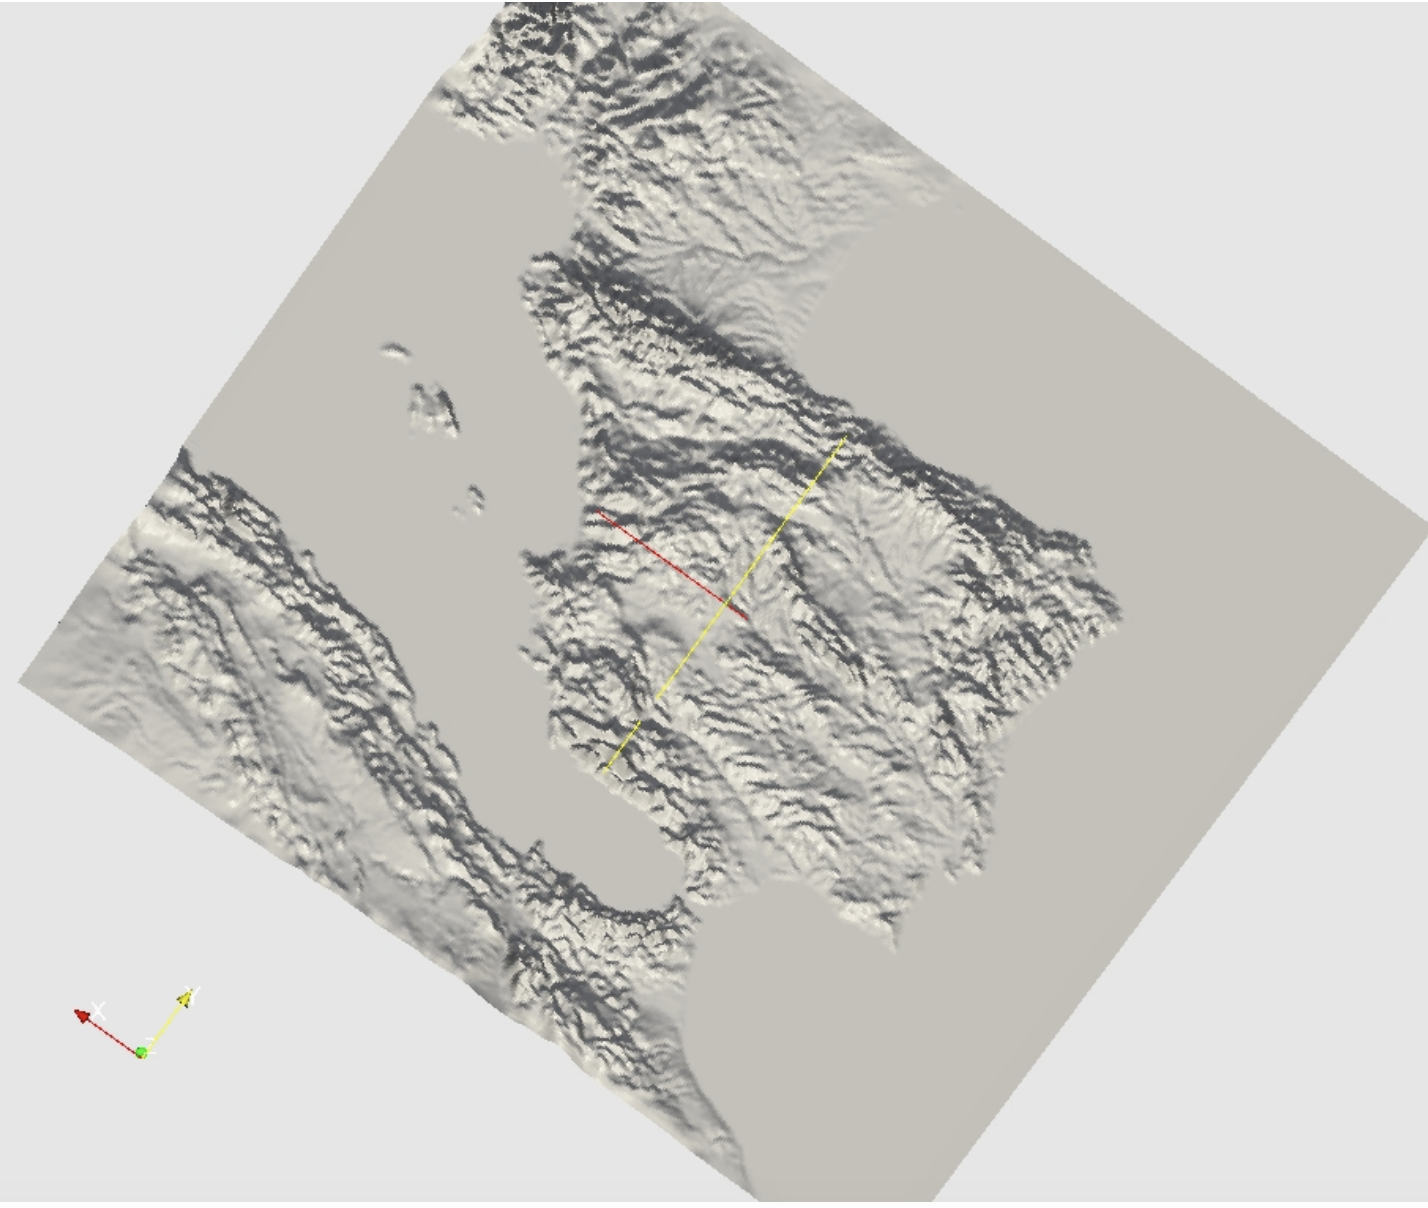
\includegraphics[width=3in]{mmesh3d_spain_surface_grid.png}
\caption{Surface grid of iberian peninsula using MMesh3d.}
\label{fig:spainSurfaceGrid}
\end{figure}

\section{Test cases}
\hl{Should this section be kept in this document or should test cases be described elsewhere?}
\subsection{Rising thermal bubble in a saturated atmosphere}
The moist dynamics is tested by means of the saturated rising bubble test described in \cite{Pressel15a}. The initial conditions are setup as follows:

\begin{itemize}
\item Initialize dry atmosphere with uniform background $\theta_{ref} = 320$ K
\item Add thermal perturbation $\Delta \theta$ of radius $r=2$ km
\item Set a uniform total mixing ratio $q_t = 0.0192 \,{\rm kg/kg}$ and $q_l = q_i = 0.0\,{\rm kg/kg}$
\item Calculate the gas constants for moist air: 
\[\begin{array}{lcl}
R_{gas} &=& {\tt MoistThermodynamics.gas\_constant\_air(q_t, q_l, q_i)}\\
c_v     &=& {\tt MoistThermodynamics.cv\_m(q_t, q_l, q_i)}\\
c_p     &=& {\tt MoistThermodynamics.cp\_m(q_t, q_l, q_i)}\\
\end{array}
\]
\item  Compute $\theta$, $\rho$, and $T$ as if the background were dry:\\
    \[ \begin{array}{lcl}
  \theta &=& \theta_{ref} + \Delta\theta\\
 \pi & =& 1 - gz/(c_p\theta)\\
 \rho & = & p0/(R_{gas}\theta)\pi^(c_v/R_{gas})\\
 T   & = &\pi \theta
\end{array}\]

\item Add the contribution of moisture to the internal energy and recalculate $T$ and $P$, and obtain $e^{\rm tot}$ using the following {\tt MoistThermodynamics} functions:
\[\begin{array}{lcl}
I &=& {\tt MoistThermodynamics.internal_energy(T + T_0, q_t, q_l, q_i)}\\
T &=& {\tt MoistThermodynamics.air_temperature(I, q_t, q_l, q_i)}\\
P &=& {\tt MoistThermodynamics.air_pressure(T - T_0, \rho, q_t, q_l, q_i)}\\
e^{\rm tot} &=& {\tt MoistThermodynamics.total_energy(0.5\|{\bf u} \|^2, gz, T, q_t)}
\end{array}\]
\end{itemize}

\hl{As of now, the saturation adjustment diverges on this initial condition. To be checked.}

\subsection{External sounding}
The current version of Cahttps://www.overleaf.com/2425712669sdzjdvvwvstsnary (\hl{A pull request from my fork was submitted yesterday to the main Canary repo}) contains the reader of an external sounding. The sounding of the test case in \citet{kurowskiEtAl2013} was added.


\section{Subgrid Scale Models}
\label{sec:sgs_models}

Subgrid-scale models for ``physics'' such as radiative transfer, microphysics, and convection parameterizations for coarse-resolution configurations are discussed in a separate document. Here we focus on SGS filters needed at any resolution, including LES resolutions \hl{(if we need them at all \dots).}


\section{Computing Aspects}
\label{sec:computing_aspects}

Let us decompose the computing aspects into the following groups
\begin{enumerate}
\item parallelization API
\item many-core API
\item graph-partitioning and grid generation

\end{enumerate}

\subsection{Parallelization API}
We propose to use the Message-Passing Interface (MPI) for communicating across processors and nodes (with multiple processors).  One of the NPS team members (Lucas Wilcox) has written Julia wrappers for MPI.

\subsection{Many-core API}
\label{sec:computing_aspects/manycore}
We propose to use a GPU library for accessing the GPUs. The NPS team has vast experience in this area. For example, the NPS team ported NUMA using OCCA2 with a CUDA back-end to run on the Titan supercomputer using 16,000 GPU cards achieving very good weak scaling \citep{abdi:2016b,abdi:2018}. The approach will be to write all of the compute-kernels in either GPUArrays (from Julia), OCCA2, or CUDA. From our perspective, the compute-kernel is the focus and most GPU-ready kernels look more or less the same (OCCA, CUDA, and OpenCL). 

\subsection{Graph-Partitioning and Grid Generation}
One of the NPS team members (Jeremy Kozdon) has written Julia wrappers to the p4est library developed by another NPS team member (Lucas Wilcox).  We propose to use p4est for both grid-generation and graph-partitioning or Metis with a specific grid generator for both the LES and global domains. The global domain will use a cubed-sphere grid while the LES domains will use a logically Cartesian cube grid.

\subsection{Code-base Repository}
The code is maintained in Github at \url{https://github.com/climate-machine/CLIMA}.

\section{Tutorial of CliMa Kernels}
\label{sec:tutorial}

In \texttt{https://github.com/climate-machine/Canary.jl/tree/master/examples} the following three folders
\begin{enumerate}
    \item 1d$\_$kernels
    \begin{itemize}
        \item LDG1d
        \item burger1d
        \item swe1d
    \end{itemize}
    \item 2d$\_$kernels
    \begin{itemize}
        \item LDG2d
        \item euler2d$\_$set3c
        \item nse2d
        \item nse2d$\_$sgs
        \item swe2d
    \end{itemize}
    \item 3d$\_$kernels
    \begin{itemize}
        \item LDG3d
        \item euler3d$\_$set3c
        \item nse3d
    \end{itemize}
\end{enumerate}
containing various sets of governing equations can be found. 

In all the folders, the LDG files solve an elliptic equation (a Poisson equation) using the Local Discontinuous Galerkin (LDG) method.  The swe files solve the shallow water equations, the euler files solve the Euler equations using the conservation form with total energy, and the nse files solve the fully compressible Navier-Stokes equations (NSE) which are nothing more than the Euler equations with the viscous stresses solved via the LDG method.  All hyperbolic equations (burger, swe, and euler) use the discontinuous Galerkin (DG) method with a simple Rusanov flux with arbitrary order polynomial basis functions on tensor-product grids (1D line, 2D quads, and 3D hexahedra).

All of these codes are structured in the same way.  Namely, at the bottom of each JL file there is a MAIN function that contains an initial condition and runs the program.  MAIN then calls the solver (e.g., in the case of Burgers equation, it calls the function BURGER, in the case of shallow water, it calls the SWE, in the case of Navier-Stokes, it calls the function NSE).  In turn, the solver function calls LOWSTORAGERK which is the time-integration loop and a proxy for any time-integrator that will be included in CliMa in the future (e.g., Additive Runge-Kutta methods for 1D-IMEX and 3D-IMEX).
The heart of all these kernels is in the LOWSTORAGERK function which looks as follows
\begin{algorithm}
\label{alg:Time-Stepper}
\begin{algorithmic}
\Function{LOWSTORAGERK}{}
\For{$step=1:nsteps$} \Comment go over time-steps
\For{$s=1:length(RKstages)$} \Comment go over multi-stages
\State 1ST$\_$ORDER$\_$OPERATOR \Comment use Alg. \ref{alg:first_order_operators}
\If{viscosity>0}
\State 2ND$\_$ORDER$\_$OPERATOR \Comment use Alg. \ref{alg:second_order_operators}
\EndIf
\State UPDATESOLUTION!() \Comment update the solution field q
\EndFor 
\EndFor
\EndFunction
\end{algorithmic}
\end{algorithm}
where it builds the first order operators and then, if required, the second order operators.  The function UPDATESOLUTION    updates the solution for the next time-step.  

The first order operators are described in Alg.\ \ref{alg:first_order_operators} below.
\begin{algorithm}
\label{alg:first_order_operators}
\begin{algorithmic}
\Function{1ST$\_$ORDER$\_$OPERATOR}{}
\State SENDDATA$\_$Q() \Comment non-blocking send of the data
\State VOLUMERHS!() \Comment compute volume integral contribution to RHS
\State RECEIVEDATA$\_$Q() \Comment non-blocking receive - for latency hiding
\State FLUXRHS!() \Comment compute flux integral contribution to RHS
\EndFunction
\end{algorithmic}
\end{algorithm}
The SENDDATA and RECEIVEDATA functions exchange the information on the CPU and/or GPU and need to be called separately in order to overlap communication with computation (we send the data and while it is being sorted out, we compute the volume integrals which require no neighbor data).  Once we finish with the volume integrals (VOLUMERHS), we then wait to receive all the data (RECEIVEDATA$\_$Q) before we compute the flux integrals (FLUXRHS), which do require neighbor data. The "!" at the end of some of the function calls denotes that the state vector $q$ or $RHS$ is modified by that function.

If second order differential operators are required (say for diffusion), then this is done after the 1st order operators as follows
\begin{algorithm}
\label{alg:second_order_operators}
\begin{algorithmic}
\Function{2ND$\_$ORDER$\_$OPERATOR}{}
\State VOLUMEGRAD!() \Comment compute volume integral contribution to $\nabla q$
\State FLUXGRAD!() \Comment compute flux integral contribution to $\nabla q$
\State UPDATEGRAD!() \Comment update the solution to compute gridpoint $\nabla q$
\State SENDDATA$\_$GRADQ() \Comment non-blocking send - for latency hiding
\State VOLUMEDIV!() \Comment compute volume integral contribution to $\nabla \cdot (\nabla q)$
\State RECEIVEDATA$\_$GRADQ() \Comment non-blocking receive - for latency hiding
\State FLUXDIV!() \Comment compute flux integral contribution to $\nabla \cdot (\nabla q)$
\EndFunction
\end{algorithmic}
\end{algorithm}
Algorithm \ref{alg:second_order_operators} uses the local discontinuous Galerkin (LDG) method to construct 2nd order operators. We have used this approach for representing 2nd order operators because it is simpler to understand since it does so by first approximating the gradient of the function (VOLUMEGRAD and FLUXGRAD) and then computing the divergence of the gradient of the function (VOLUMEDIV AND FLUXDIV).  

%-------Bibliography
\bibliographystyle{agufull08}
\bibliography{Giraldo_refs,CLIMA-refs}

\end{document}
